%!TEX root = ../../../main.tex

\subsection{Pairwise-covariance Multi-view Discriminant Analysis pc-MvDA}
    MvDA emphasizes on finding a common space with minimal within-class variation while the distances between class means and global mean are jointly maximized. However, the distances between some pairs of classes can be disregarded. In this paper, to obtain this property, we modified MvDA with reformulated between and with-in class scatter matrices terms in a pairwise manner. First, let us define a new inter-class scatter matrix formula that takes paired distance into account:
    \begin{equation}
        \boldsymbol{S}_B^y=\sum_{a=1}^{c}\sum_{b=a+1}^{c}{\left(\mu_a-\mu_b\right)\left(\mu_a-\mu_b\right)^T}
    \end{equation}
    where $a$, $b$ are two distinct classes. For each pairs of class $a$ and class $b$, the between covariance is calculated as:
    \begin{equation}
        {\boldsymbol{S}_B^y}_{ab}={\left(\mu_a-\mu_b\right)\left(\mu_a-\mu_b\right)^T}
        \label{eq:Sb_ab}
    \end{equation}

    The intra-class scatter matrix $\boldsymbol{S}_W^y$ of MvDA is calculated as simple summation of all covariance matrices of each $i^{th}$ class, $i = {1,...,c}$:
    \begin{equation}
        {\boldsymbol{S}_W^y}_i=\sum_{j=1}^{v}\sum_{k=1}^{n_{ij}}{\left(y_{ijk}-\mu_i\right)\left(y_{ijk}-\mu_i\right)^T}
    \end{equation}

    Mathematically, it assumes data samples from each class among all views are identically Gaussian distributed, and contribute evenly to the minimization of intra-class scatter. In reality, it is hardly the case as data variations of samples from different classes and different view points are usually drastically diverse and may also have different dimensions.

    To better represent the distribution of data, pc-MvDA uses a paired intra-scatter matrix which is denoted as
    \begin{equation}
        {\boldsymbol{S}_W^y}_{ab}=\beta\frac{n_a{\boldsymbol{S}_W^y}_a+n_b{\boldsymbol{S}_W^y}_b}{n_a+n_b}+\left(1-\beta\right){\boldsymbol{S}_W^y}
        \label{eq:Sw_ab}
    \end{equation}
    where $0\le\beta\le1$ is a hyper-parameter for regularization between the original global intra-covariance ${\boldsymbol{S}_W^y}$ and the novel two local class covariances ${\boldsymbol{S}_W^y}_a$ and ${\boldsymbol{S}_W^y}_b$. This formulation is closer to the value of covariances of both classes than the standard intra-covariance.

    Instead of solving the vanilla generalized eigen value problem for the whole dataset, we split it into sub-problems for each pairs of class $a$ and $b$, in which we define the objective distance to be minimized between two corresponding classes.
    \textbf{Difference of our proposed method compared to pairwise LDA (pc-LDA)}
    In pc-LDA \cite{kong2014pairwise}, the pairs of $a$ and $b$ classes are regarded as two Gaussian distributions $\mathcal{N}_a(\mu_a,{\boldsymbol{S}_W^y}_a), \mathcal{N}_b(\mu_b,{\boldsymbol{S}_W^y}_b)$ and the objective distance between two classes is defined as their Kullback-Leibler divergence \cite{kullback1951}:
    \begin{equation}
        D_{KL}\left(\mathcal{N}_a\parallel\mathcal{N}_b\right)=\frac{1}{2}\left(\mu_a-\mu_b\right)^{T}{\left({\boldsymbol{S}_W^y}_{ab}\right)}^{-1}\left(\mu_a-\mu_b\right),
    \end{equation}
    Then the final objective is properly weighted to focus on classes with more samples:
    \begin{equation}
        \operatorname*{min}_{\boldsymbol{\omega}_1, \boldsymbol{\omega}_2,...,
        \boldsymbol{\omega}_v}{J}=\sum_{a=1}^{c}\sum_{b=a+1}^{c}{\frac{n_an_b}{{[2D_{KL}\left(\mathcal{N}_a\parallel\mathcal{N}_b\right)]}^q}}
        \label{eq:pc-LDA}
    \end{equation}
    here $q\ge1$ is a hyper-parameter that controls how much the pairs of classes with smaller objective distances are biased over the others.

    In our observation, the minimization of KL divergence for each pairs of classes $a$ and $b$ can be substituted by a generalized eigenvalue problem with the pairwise ${\boldsymbol{S}_W^y}_{ab}$ and the ${\boldsymbol{S}_B^y}_{ab}$ we defined. Although these sub-problems do not have an unified analytical solution to be solved concurrently, the criteria can be formulated in various differentiable ways like in \cite{fukunaga1990441} so we can use gradient descent algorithm:
    \begin{equation}
        J_1=\frac{tr(S_B)}{tr(S_W)};\quad 
        J_2=tr\left(\frac{S_B}{S_W}\right);\quad
        J_3=tr\left|\left|\frac{S_B}{S_W}\right|\right|;\quad
        J_4=\frac{det(S_B)}{det(S_W)}
    \end{equation}

    We choosed the former Fisher loss as the ratio of scalar values is computationally cheaper. Comparing to the objective of pc-LDA in Eq.\eqref{eq:pc-LDA}, our proposed model is obviously more efficient since it contains only simple operators and the need to inverse a singular-prone matrix is negated. Therefore, it is better fit in the scenario where we want to train the model multiple iterations over multi-view high dimensional output.

    Our final objective function of pairwise-covariance multi-view discriminant analysis is sum of all pairwise Fisher criteria with normalized weights:
    \begin{equation}
        \operatorname*{min}_{\boldsymbol{\omega}_1, \boldsymbol{\omega}_2,..., \boldsymbol{\omega}_v}{J}=\sum_{a=1}^{c}\sum_{b=a+1}^{c}{\frac{n_an_b}{n_{cc}^2}{\left[{\frac{trace\left({\boldsymbol{S}_W^y}_{ab}\right)}{trace\left({\boldsymbol{S}_B^y}_{ab}\right)}}\right]}^{q}}
        \label{eq:pc-MvDA}
    \end{equation}
    where $n_{cc}$ is the number of common components as coined in \cite{you2019multi} or simply number of samples in each view. This added normalization term assures that the objective does not depend on size of dataset.

    Let's look at the Fig.\ref{fig:frw}, the nominator of MvDA(-vc) $\boldsymbol{S}_B^y$ is the sum of all distances from mean of every class $\mu_i$, $i = {1,...,c}$ to the mean of all classes $\mu$. This helps to push class far away from the mean of all classes (the dotted green lines in Fig.\ref{fig:frw}). However, it may not ensure that the classes will be far from each other (Fig.\ref{fig:pc-MvDA}a). In this work, we take the pairwise distance into account and integrate them in an multi-view framework (the dotted violet lines in Fig.\ref{fig:frw}). Thanks to this, the classes will be more discriminated (Fig. \ref{fig:pc-MvDA}b). The algorithm for solving pc-MvDA is presented in supplemental materials. 

    \paragraph{Illustrative examples}
        We illustrate the advantage of pc-MvDA on artificial datasets. Firstly, using function provided by scikit-learn library, we generate several isotropic Gaussian blobs equal to desired number of classes as data samples from one single view. To generate other views, we clone and apply translation, point-wise noise and rotation with random orthogonal group multiplication to the first view.

        \begin{figure}[htbp]
            \centering
            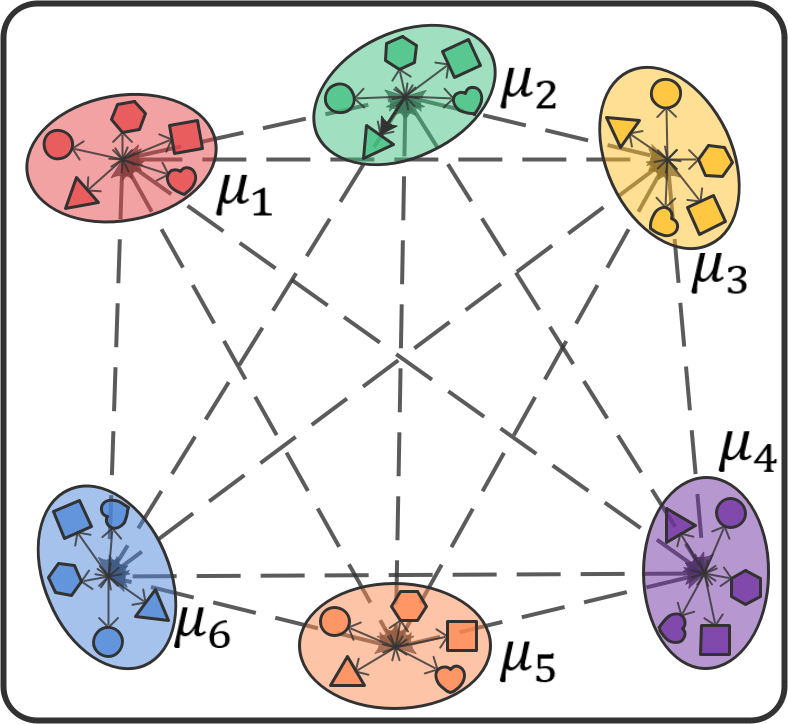
\includegraphics[width=0.7\linewidth]{Figs/pc-MvDA.png}
            \caption{a) MvDA does not optimize the distance between paired classes in common space. b) pc-MvDA takes pairwise distances into account then distinguish better the classes.}
            %\vspace{-0.3cm}
            \label{fig:pc-MvDA}
        \end{figure}

        In Fig.\ref{fig:synthetic1}, MvDA and pc-MvDA results on 2D synthetic dataset of 180 data points in 2-D space. There are three classes, observed at three viewpoints. We show data distribution and 1-D projection results using MvDA and pc-MvDA respectively. We notice that data points of two classes (the first and the third classes) are close together in original space. When we project in common space by MvDA, these classes are still close together. In contrast, these classes are more discriminant when projected by pc-MvDA.

        \begin{figure}[htbp]
            \centering
            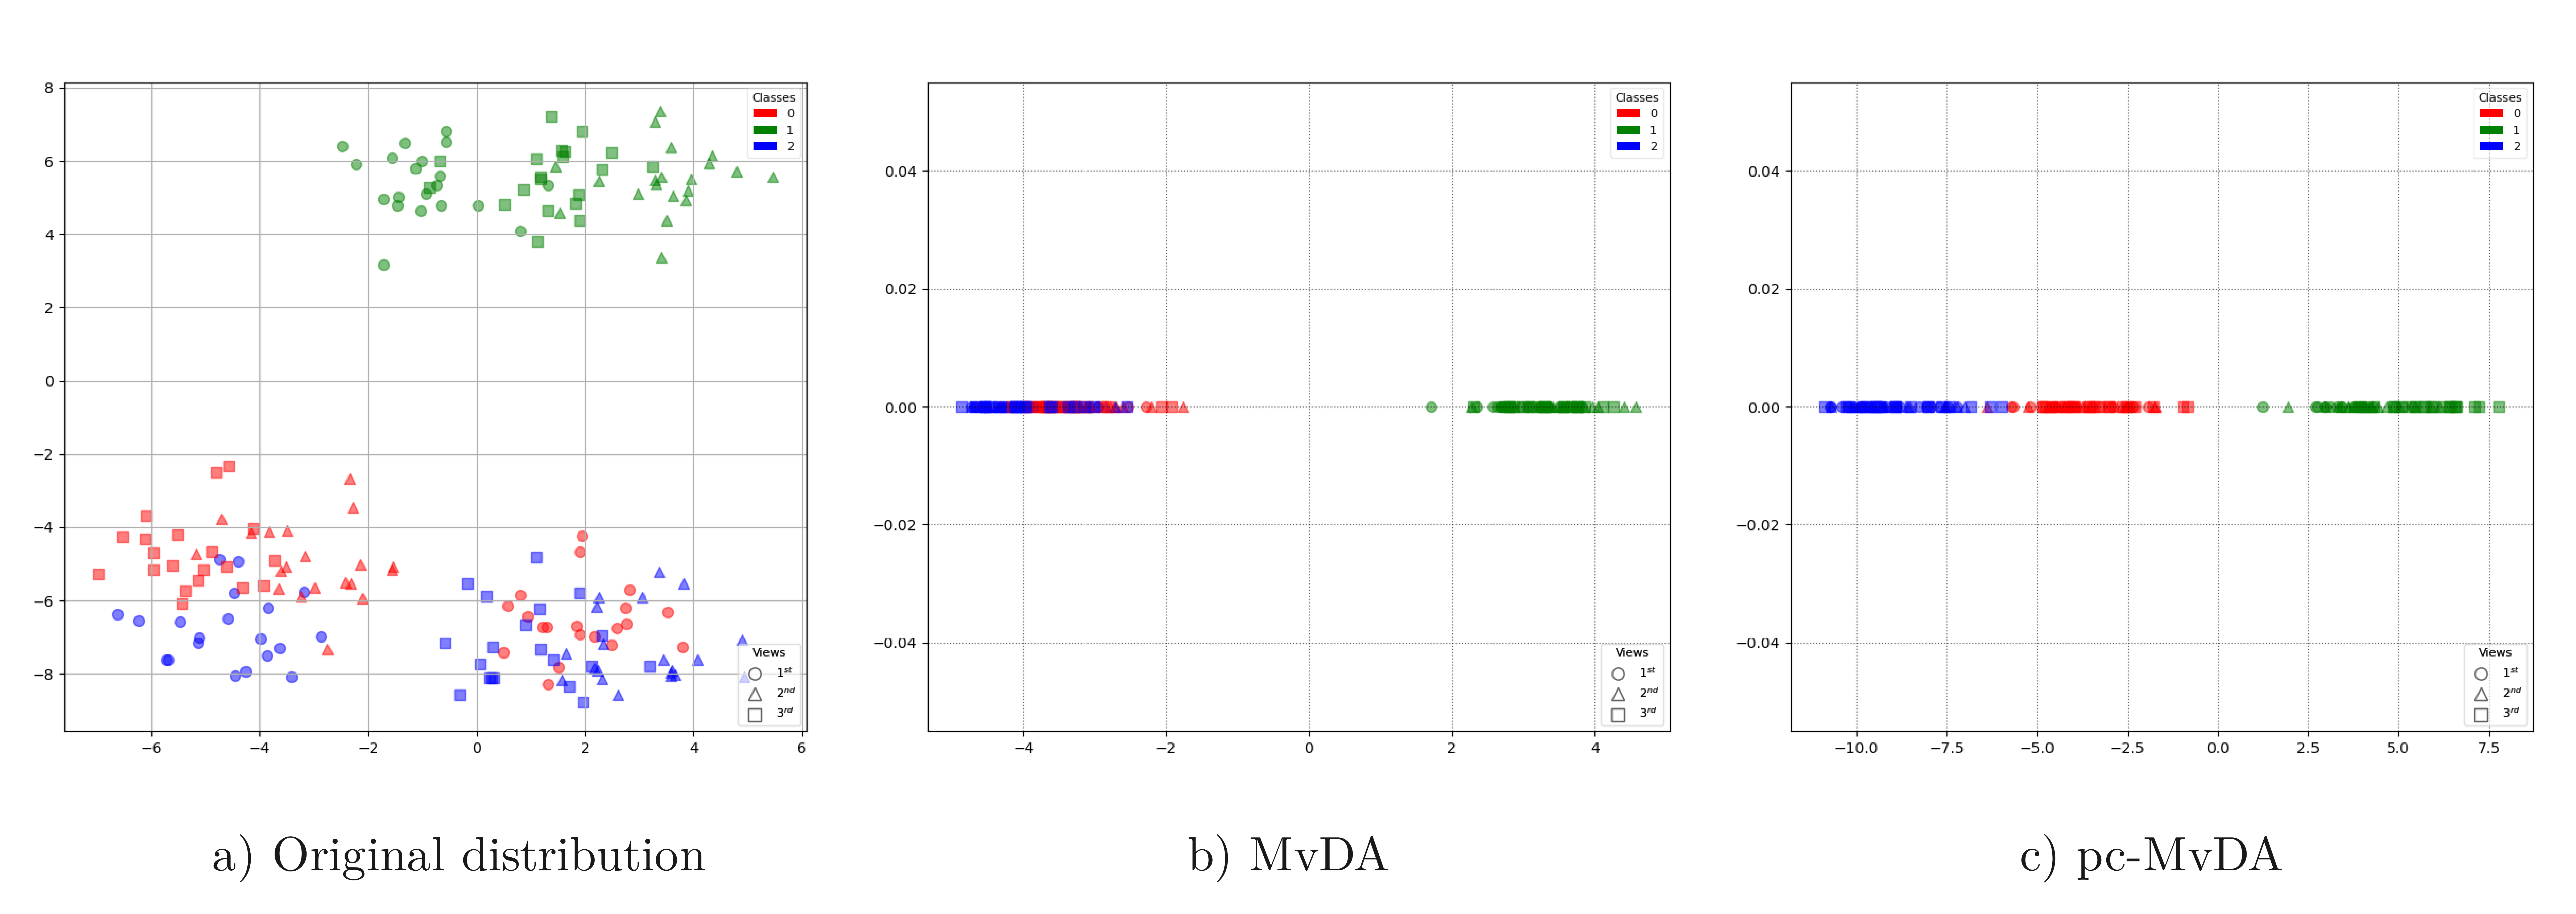
\includegraphics[width=1\linewidth]{Figs/Synthetic1.png}
            \caption{A synthetic dataset of 180 data points, evenly distributed to 3 classes among 3 different views; a) 2-D original distribution; b) 1-D projection of MvDA; c) 1-D projection of pc-MvDA}
            %\vspace{-0.3cm}
            \label{fig:synthetic1}
        \end{figure}

        Similar to the first example, in the second example, we generate 300 data points of 5 classes observed from 3 different views (Fig.\ref{fig:synthetic2}). We observe that the five clusters of pc-MvDa common space contract strongly and become more separated as compared to the MvDA results (especially the first and the fourth classes).

        \begin{figure}[htbp]
            \centering
            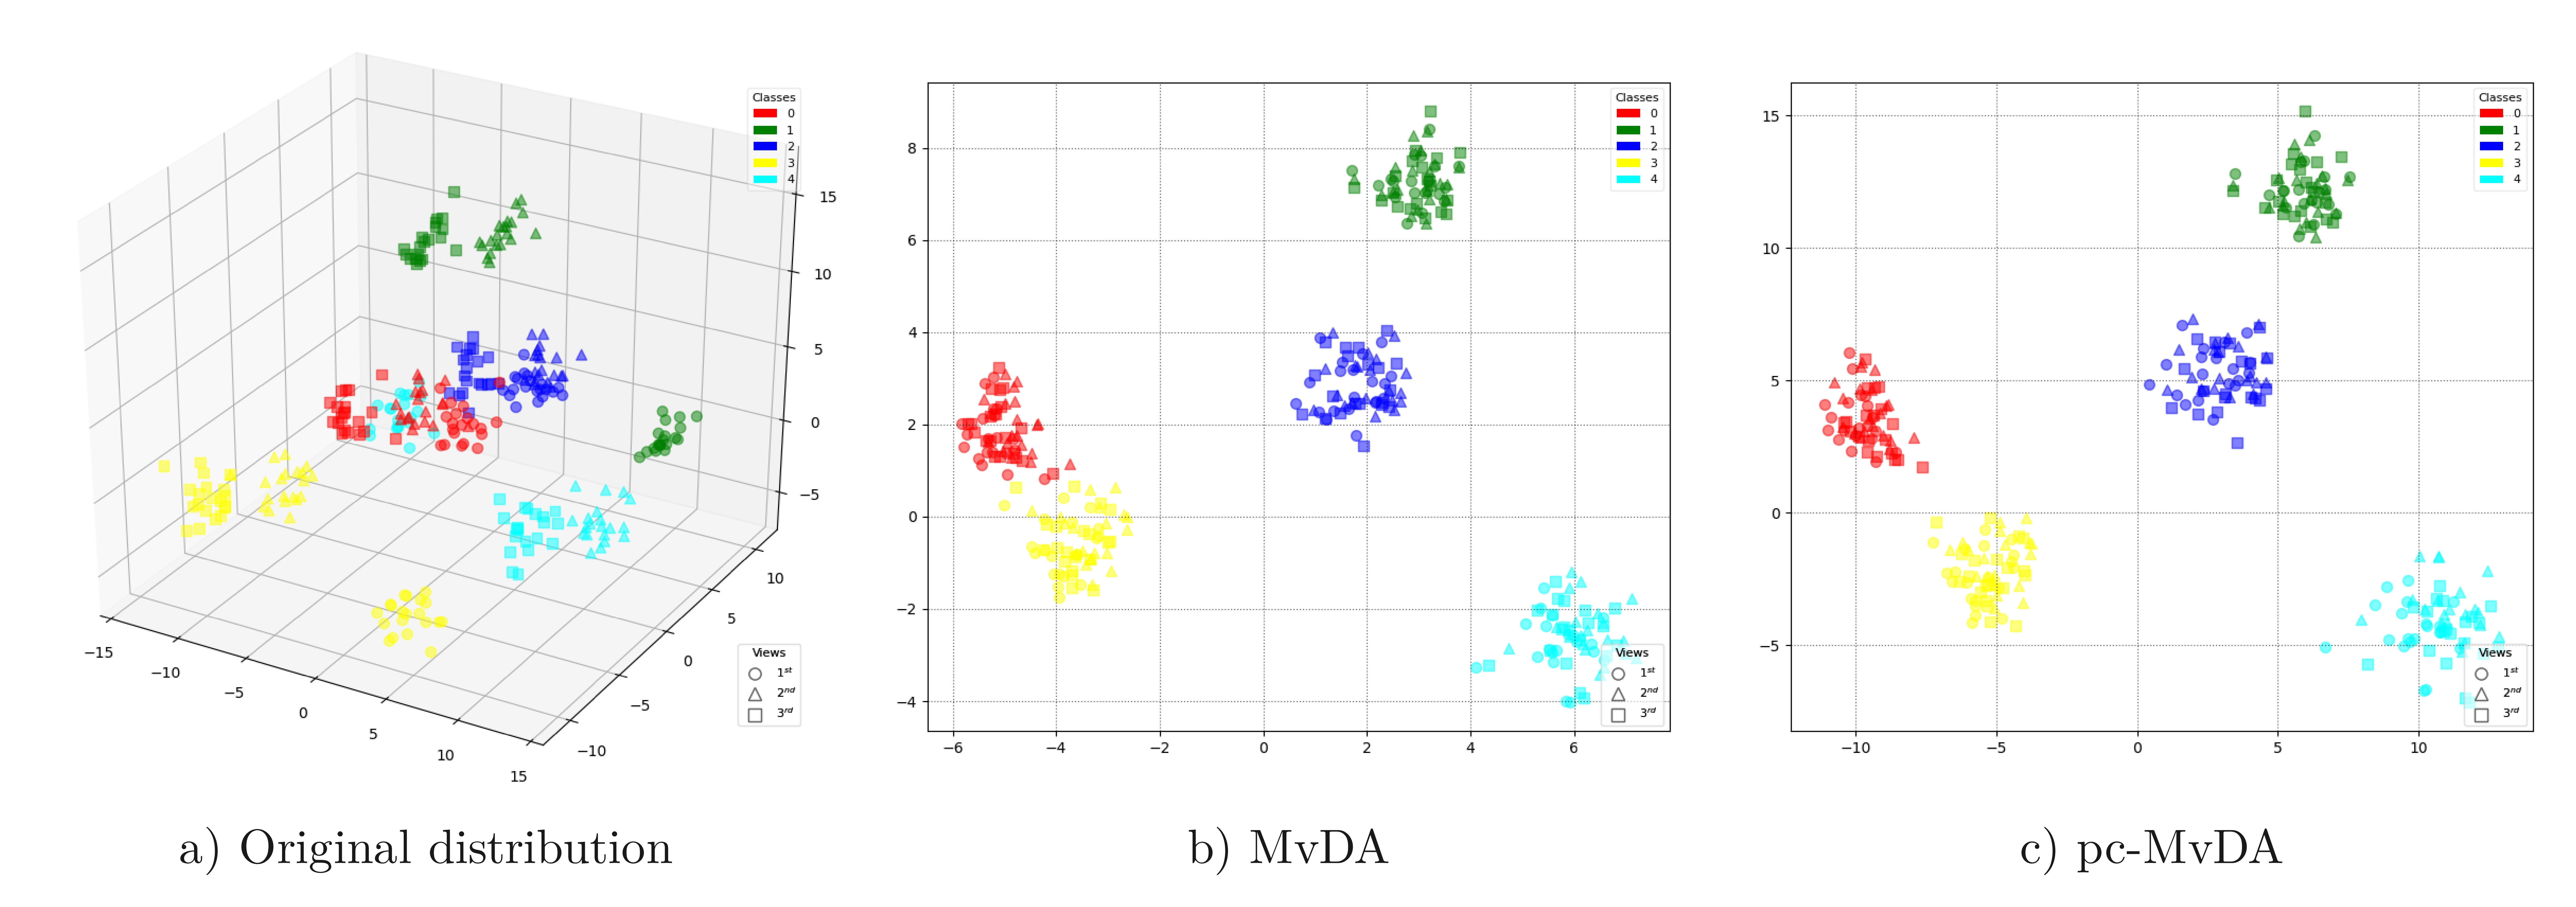
\includegraphics[width=1\linewidth]{Figs/Synthetic2.png}
            \caption{A synthetic dataset of 300 data points, evenly distributed to 5 classes among 3 different views; a) 3-D original distribution; b) 2-D projection of MvDA; c) 2-D projection of pc-MvDA}
            %\vspace{-0.3cm}
            \label{fig:synthetic2}
        \end{figure}

    \paragraph{Algorithm to solve pc-MvDA}
        As the proposed objective does not match any optimization form of generalized eigenvalue problems, gradient descent algorithm is used to solve pc-MvDA. This approach also allow the algorithm to update incrementally even in higher dimensional data where the computations of matrix inversion and eigenvectors are not conducive. The derivative of Eq.\eqref{eq:pc-MvDA} is:

        \begin{equation}
            \frac{\partial J\left(W\right)}{\partial W}=-\sum_{a<b}^{c}{\frac{qn_an_b}{{n_{cc}}^2{J_{ab}\left(W\right)}^{q+1}}\frac{\partial J_{ab}\left(W\right)}{\partial W}}
        \end{equation}

        where $J_{ab}\left(W\right)={tr\left({\boldsymbol{S}_B^y}_{ab}\right)}/{tr\left({\boldsymbol{S}_W^y}_{ab}\right)}$ is the Fisher loss of class pair $a$ and $b$. Its gradient is computed using the funky trace derivative and quotient rule:

        \begin{equation}
            \frac{\partial J_{ab}\left(W\right)}{\partial W}=\frac{tr\left({\boldsymbol{S}_W^y}_{ab}\right)W^T\left({\boldsymbol{S}_B^x}_{ab}+{{\boldsymbol{S}_B^x}_{ab}}^T\right)-tr\left({\boldsymbol{S}_B^y}_{ab}\right)W^T\left({\boldsymbol{S}_W^x}_{ab}+{{\boldsymbol{S}_W^x}_{ab}}^T\right)}{{tr\left({\boldsymbol{S}_W^y}_{ab}\right)}^2}
            \label{eq:grad_Jab}
        \end{equation}

        The superscript $x$ replacing $y$ in scatter matrices notations means that they denote the pre-transformed version. With simple algebra, we can rewrite the formulas in matrix multiplication form, separating transformation vectors $\omega_j$ in a concatenated matrix $W$ and a multi-view covariance matrix constructed from $v\times v$ cells, each cell $S_{jk}$ stands for the covariance between view $j$ and view $k$.

        \begin{equation}
            \boldsymbol{S}^y=W^T\boldsymbol{S}^xW=\left[\begin{matrix}\omega_1^T&\omega_2^T&\cdots&\omega_v^T\\\end{matrix}\right]\left[\begin{matrix}S_{11}&S_{12}&\cdots&S_{1v}\\S_{21}&S_{22}&\cdots&S_{2v}\\\vdots&\vdots&\ddots&\vdots\\S_{v1}&S_{v2}&\cdots&S_{vv}\\\end{matrix}\right]\left[\begin{matrix}\omega_1\\\omega_2\\\vdots\\\omega_v\\\end{matrix}\right]
        \end{equation}

        The complete algorithm to compute $\nabla J$ is given in Algorithm \ref{algo:grad_computation}.

        \begin{algorithm}
            \SetKwInOut{Input}{Input}
            \SetKwInOut{Output}{Output}
            \SetEndCharOfAlgoLine{\relax}
            \Input{$W$, \{$X$, $\mu$\}, $q$}
            \Output{$\nabla J\left(W\right)$}
            $\boldsymbol{F} = 0$\;
            Compute $\boldsymbol{S}_W^x$ according to Eq.\eqref{eq:MvDA_Sw}\;
            \For{$a=1$ \KwTo $c$} {
                \For{$b=a+1$ \KwTo $c$} {
                    Compute ${\boldsymbol{S}_B^x}_{ab}$ according to Eq.\eqref{eq:Sb_ab}\;
                    Compute ${\boldsymbol{S}_W^x}_{ab}$ according to Eq.\eqref{eq:Sw_ab}\;
                    Compute ${\boldsymbol{S}_B^y}_{ab}=W^T{\boldsymbol{S}_B^x}_{ab}W$\;
                    Compute ${\boldsymbol{S}_W^y}_{ab}=W^T{\boldsymbol{S}_W^x}_{ab}W$\;
                    Compute $J_{ab}=tr\left({\boldsymbol{S}_B^y}_{ab}\right)/tr\left({\boldsymbol{S}_W^y}_{ab}\right)$\;
                    Compute $\nabla J_{ab}$ according to Eq.\eqref{eq:grad_Jab}\;
                    $\boldsymbol{F} = \boldsymbol{F} + n_an_b\nabla J_{ab}/J_{ab}^{q+1}$\;
                }
            }
            $\nabla J = {-q\boldsymbol{F}}/{n_{cc}^2}$\;
            \Output{$\nabla J$}
            \caption{Computation of $\nabla J\left(W\right)$ (i.e. gradient of Eq.\eqref{eq:pc-MvDA})}
            \label{algo:grad_computation}
        \end{algorithm}

        No further constraint is imposed to the model. In my implementation of pc-MvDA in Pytorch, the computation of gradient is in fact handled by automatic differentiation. I choose Adam as optimizer with learning rate set to $0.01$. To have better starting point and mitigate variances, pc-MvDA is initialized with transformation learnt by MvDA.
